%!TEX root = ../report.tex

\section{Definitions}


%add refferences

%[REF] Survey of software refactoring tools \cite{erb2010survey}
This section presents some definitions regarding refactoring activities.

\subsection{Classification of the refactoring}
There are several levels of refactoring, from a high-level refactoring, like design refactoring, to a low-level refactoring such as the extract method refactoring operation.
In between, exists combinational refactoring that is a combination of several low level refactoring operations.
Refactoring operations can also be classified by the effect they have on software quality attributes.
In order to classify the effect based on software quality attributes, it is necessary to map the changes in the internal software quality metrics, e.g. lines of code, cohesion or coupling, to the external software quality attributes, e.g. adaptability, reusability or testability. \cite{elish2011classification}
However, this is a complex task that is outside the scope of this thesis and therefore it will not be further detailed.

%(i) internal software quality metrics and (ii) external software quality attributes (adaptability, completeness, maintainability,
%understandability, reusability and testability). The classification is done by mapping the changes in the
%internal quality metrics, caused by applying refactoring methods, to the external quality attributes.

\subsection{Refactoring as a Process}
Refactoring can be done in two ways. %add citations
One is doing the refactoring in between programming and constantly performing it.
The other one is to do the refactoring as a separate activity and done in bulk.
Regardless when is done, the refactoring can always be decomposed in different activities: \cite{erb2010survey}

\begin{enumerate}
 \item Identify where to change the software
 \item Determine the adequate refactoring operation
 \item Have a way to protect the planned changes (e.g, automated tests)
 \item Make the planned changes
 \item Access the refactoring benefits
 \item Maintain consistency between refactored and non-refactored code
\end{enumerate}


%Eisenecker et al. [2000] defined requirements for the refactoring tools

%Functional requirements of a refactoring tools:
%Image, or explain in text => explain in text
%Non Functional requirements of a refactoring tool:
%Image. or explain in text.

\subsection{Refactoring Correctness}
%survey of software refactoring tools \cite{erb2010survey} %add citation
%
Refactoring must preserve the program's behavior in order to be correct.
However, there is no consensual definition for what behavior preservation is.
Some authors say that the behavior of the program is the output and preserving the input-output behavior preserves the program behavior suggested by Opdyke \cite{opdyke1992refactoring}.
However, other authors think that preserving the output is insufficient, since other aspects may be relevant as well. For example, for real-time software, the execution time of certain operations is an important aspect of the behavior.
One way to deal with behavior preservation is to have an extensive set of test cases and if all these tests still pass after the refactoring, it is highly probable that the refactoring is correct \cite{mens2004survey}.
A more formal approach is to prove that the refactoring operations preserve the full program semantics. For Prolog, that has simple and formally defined semantics, it is simple to prove that refactoring preserve the program semantics \cite{proietti1991semantics}. %27?
But for more complex languages such as C++, which the formal semantics is extremely difficult to define, typically it is necessary to put restrictions to the refactoring operations or to the language constructs and the refactoring tool may be limited to a particular version of a particular compiler \cite{tokuda2001evolving}.%28?
% \cite{mens2004survey}.

%For example in a class, if a method name is renamed and the program consists in printing that method name, by renaming that method the behavior of the program changes.

%Another way do define it is to say that in order to preserve behavior it is necessary to preserve the syntactically and semantic properties.
%Preserving the syntactic properties is to still have a well-formed program after the transformation, and it is common sense that a refactoring should not invalidate a syntactic correct program.

%Preserving the semantics of the program means to preserve the meaning of the program in the basic concept of the language.
%In other words, the semantic properties of all declarations after a refactoring should resolve to the same declarations they resolved before the transformation.
%Because preserving the syntax is easily seen, this document focus on the meaning-preservation of the refactoring operations.


%suvey mens 2003 \cite{mens2003refactoring}
%What is behaviour and how to preserve it?
%Observational behaviour, for the same input we get the same output, is not always sufficient.
%for example, for Real time systems it is important the time that a (sequence of) operations takes, for embedded systems it takes into account the memory and the power consumption and for safety-critical systems there is a defined safety that must be preserved.
%In a theoretical world all this properties should be preserved by a refactoring, however in practice that is not the case.

\subsection{Case Study - Manual Refactoring}

One way to learn how the users manually refactor is to do it while taking notes.
%The case study \cite{thompson2003case} was done with the idea to show that refactoring is also important in functional programs.
The case study \cite{thompson2003case} consists in refactoring an Haskell program with 400 lines, written by a student.
The program's goal is to build a semantic tableaux, which is a truth tree used for example to proof procedures for first order logic or solve satisfiability of finite sets.

%\subsubsection{Refactoring of a program}
In order to better understand in what consists a refactoring they applied manual refactoring operations to the program.
They started by changing the name of some variables to avoid misunderstandings and to be easier to read.
After that they renamed some functions to names that reflect better what the function did.
Then they replaced explicit recursion by calls to higher order functions and they rename some variables and functions.
In the end they generalized some functions and modified the representation type because it was giving a lot of work keeping the initial representation.

%\subsubsection{What was learned}
This case study shows that the order of the refactoring operations is somehow arbitrary.
The refactoring operations were applied whenever they thought it made more sense.
They also conclude that generally, refactoring a program is a good way to find out more about the program.
And that the refactoring operations need to have a way of doing undo, redo or revert changes, otherwise it would be more difficult to correct mistakes.

It is crucial to document the refactoring operations applied in detail.
This aspect was stressed because having documentation about the version previous to the refactoring, or outdated, is not good for the readability of the program since it can mislead the programmer.


\subsection{Classification of refactoring tools} %\cite{erb2010survey}
Refactoring tools can be subdivided in manual, semi-automated and fully-automa\-ted according to the degree of automation.
In the manual case there is no support for detecting refactoring opportunities, but the transformation is applied by the refactoring tool. If the transformation itself is left to the user, the tool can not be considered a refactoring tool.
The fully-automated one, automatically identifies refactoring opportunities and automatically applies them.
Finally the semi-automated one identifies refactoring opportunities but waits for the user to decide the application of the refactoring.



%\subsection{Levels of Refactoring}
%There are different kinds of refactoring.
%There is manual, that is refactoring without tool support.
%Syntactic, refactoring only focused on the syntax transformations.
%Semantic, the most common one, takes into account the syntactic and semantic information in the transformations.
%And finally there is the Automated, that automatically detects the possible refactoring operations to be applied.


% subsubsection subsubsection_name (end)

\subsubsection{Manual Refactoring Tool}
is a refactoring tool that applies the refactoring operations selected by the user.
Is available for all kind of languages and it is the most common level of refactoring.
%Besides that, and in contrast with the object oriented languages, there is a lack of semantic refactoring tools for dynamic languages.
There are several examples of this tools, including Eclipse and IntelliJ that are focused in static languages and for dynamic languages there is the refactoring browser for Smalltalk.
This kind of tools will be further detailed in the related work section.
%Semi-Automated Application   & The Refactoring Browser \cite{roberts1997refactoring}, Griswold \cite{griswold1993automated} \\ \hline
%\subsubsection{Syntactic refactorings}
%prof paper

%In this paper \cite{leitdo2002formal} it is proposed a pattern language refactoring tool that works well on lisp-like languages.

%The pattern is composed by transformations that are described in a simple syntax and even that the pattern is composed by operations of simple syntax they are composable, which makes it easier for the programmer to extend the refactoring tool, and there is no impediment to create complex transformations.

%The tool also can induce transformation rules based on manual examples given by the programmer and then if needed the programmer can easily extend those rules.

%This tool is simple because it is focused on syntax transformations of the program.
%Meaning that it does not need semantic information such as bindings relations needed for transformations, making it a simpler tool.


\subsubsection{Semi-Automated Refactoring Tool}
is a refactoring tool that suggests refactoring opportunities to the user and applies the refactoring operations that the user selected.
In order to know what refactoring operations to do, the tools can use metrics that can support the decision of where and which refactoring operations to apply.
The tool \cite{simon2001metrics} was created as proof of concept and it uses the metrics to identify where the code should be refactored.
The tool takes into account the "bad smell" of a code to suggest a refactoring.
A "bad smell" is a human intuition in which a specific code should be refactored.
An example of a ``bad smell'' that trigger a Move method refactoring, which moves a method from one location to another, occurs when one method is used more by other class than the class in which the method is defined.

%An example of a "bad smell" that would trigger a Move Method refactoring, that moves a method from one location to another, is when one method of a class is used more by other class in which it is defined.

To quickly show to the user the identified "bad smells" a visualization of the methods and attributes is generated and those objects are linked to the corresponding source code, as it can be seen in the Figure~\ref{fig:MetricsBasedRefactoring}.

\begin{figure}[h!]
  \centering
  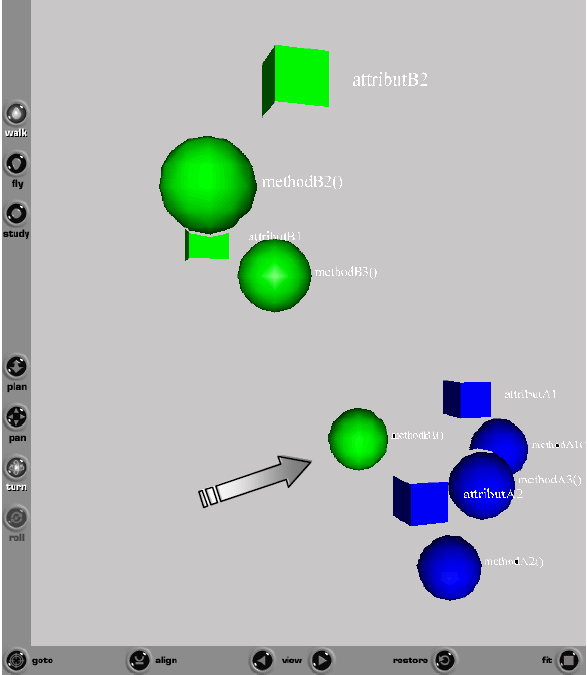
\includegraphics[width=0.75\textwidth]{img/metricsbasedrefactoring.png}
  \caption{Motivates the refactoring move method}
  \label{fig:MetricsBasedRefactoring}
\end{figure}

%\subsubsection{Distance based cohesion on refactoring operations}
In order to make an automated approach to identify "bad smells" a distance based cohesion metric is used.
With the distance based algorithm it is possible to identify violations to the rule "put together what belongs together".
There are some refactoring operations that are related to this rule such as, move attribute, extract class, in-line class and move method.
Regarding the distances, a method using only locally defined methods or attributes has a high distance to the methods of other classes, whereas methods that use many attributes and/or methods of other classes have a low distance to them.
The attributes are compared by the methods that use them.
For example if an attribute is only used by methods of other classes, that attribute probably should be moved to a different class.

\subsubsection{Automated Refactoring Tool}
is a refactoring tool that automatically applies the refactoring opportunities that the tool detects.
This kind of tool is useful when doing a source to source transformation, eliminating features that are not necessary and translating them into equivalent ones.
For example, if there is a profiling tool that only works in the previous versions of Java 1.4 and the user wants to use such profiling tool, an automated refactoring tool can be used in order to refactor the program by translating the new features, such as anonymous classes, into equivalent ones.
However, automated refactoring tools can also be used like a normal refactoring tool but has some restrictions because the user do not know what the refactoring tool is doing.
Casais \cite{casais1994automatic} or Moore \cite{moore1996automatic} are good examples of those refactoring tools.

%finding common attributes of classes and pulling those up into new super-classes
%GURU is a fully automated  tool for refactoring inheritance hierarchies and refactoring methods in SELF programs

%refactoring automaticas, source to source, e alinguagem source tem features que nao quero tratar. e elimina essa features, eg traducao pos 1.4 to pre 1.4 classes internas anonimas. ferramenta so funciona com versao antiga eg profiling.
%Automated                    & Casais \cite{casais1994automatic} or Moore \cite{moore1996automatic}

%The automated ones are used to improve internal software quality by removing the duplication of methods and attributes. However this tools have problems in preserving the understandability.
%There is no current or little practical relevance for full-automated approaches.


\subsubsection{Analysis:}
Having the automated refactoring tool for inexperienced users is not what is intended.
Transforming automatically the program will create a new program that the user might not comprehend, especially if the user is inexperienced.

The Semi-automated tool with the suggestions would be an advantage to inexperienced users that are still learning what refactoring operations exists and that way the users would learn new refactoring operations and have programs with better quality.
However, detecting refactoring opportunities is highly dependent on the application domain, witch invalidates this type of tools since they are not meant for one type of application only.

The ideal approach is a Manual Refactoring tool that applies exactly what the user wants to do.
This type of tool do not automatically detects refactoring opportunities, but it is faster and safer than doing the refactoring operation without any support.
